\documentclass[../main/main.tex]{subfiles}
\begin{document}
\setcounter{chapter}{4}
\chapter{Modélisation hyperspectrale}\label{ch:modelhyperspec}

\minitoc
\vspace{2cm}
Ce chapitre est consacré l'étape de construction du cube intrinsèque de
la galaxie hôte, que nous avons introduit dans le
chapitre~\ref{ch:hypergal}.

Nous présenterons dans un premier temps le relevé Pan-STARRS, les images photométriques
qui serviront de base d'information pour notre modélisation hyperspectrale et les
étapes de pré-traitement à appliquer.

Puis nous introduirons le SED Fitter \pkg{CIGALE}, qui sera utilisé pour
obtenir une SED de la galaxie à l'échelle locale, la configuration
implémentée et son application aux images photométriques.

Enfin, nous détaillerons la construction du cube intrinsèque, étape
finale de la modélisation hyperspectrale de la galaxie.
\newpage

\section{Source photométrique}
\label{sec:photosource}

Notre cadre de recherche étant au sein de la collaboration ZTF, nous
devons prévoir le fait que nous aurons des alertes d'évènements
transitoire dans tout le ciel Nord, couverture de la caméra. Par
ailleurs, le but d'\hypergal étant une modélisation de scène d'une
observation de la SEDm, la source photométrique utilisée doit avoir a
minima la même profondeur en magnitude. Enfin, la projection se faisant
de l'espace photométrique vers l'espace des observables de la SEDm, il
serait plus judicieux d'utiliser un relevé photométrique attestant d'un
meilleur seeing, pour éviter de dégrader les données.

Le relevé Pan-STARRS1 du système Pan-STARRS — Panoramic Survey Telescope and Rapid
Response System - \citep{Kaiser2002,Kaiser2010} répond à tous ces critères. C'est d'ailleurs basé sur
la première Data Release ce relevé astronomique que la procédure de calibration photométrique
de ZTF est effectuée.

\subsection{Relevé astronomique Pan-STARRS1}
\label{ssec:ps1}

Le relevé Pan-STARRS1 \citep{ChambersPS1survey} est une installation innovante d’imagerie
astronomique à grand champ,
développé à l'Institut d'astronomie de l'Université de Hawaï. Le relevé
Pan-STARRS1 vient du nom du premier télescope du projet situé à l'Observatoire Haleakala,
Pan-STARRS Telescope \#1 ou encore PS1. L'optique de PS1 est décrit dans
\citet{Hodapp2004a, Hodapp2004b, Hodapp2004c, Morgan2008}.
Ce télescope possède un miroir
primaire de 1m80 de diamètre avec une focale de 8m, et un miroir
secondaire de 0.9m. 

La caméra montée sur le télescope PS1 est la Gigapixel Camera \#1
(GPC1) de $1.4$ gigapixel, conçue au laboratoire Lincoln
\citep{Tonry2006GPC1,Tonry2008GPC1} et offrant un champ de vue d'environ
$3.3\degree$ de diamètre. 
Le plan focal de la caméra GPC1 est divisé en 60 appareils OTA CCID58
(Orthogonal Transfer Array; \citet{Tonry1997OTA,Tonry2008GPC1}), où
chacun est composé d'un réseau de 8$\times$8 CCDs (cellules). Un unique
OTA est composé de 64 cellules de 590$\times$598 pixels de
$\SI{10}{\micro\metre}$ de côté. Une illustration du plan focal de la
caméra est présentée dans la Figure~\ref{fig:gpc1focalplan}.

\begin{figure}[h]
  \begin{minipage}[c]{0.4\textwidth}
    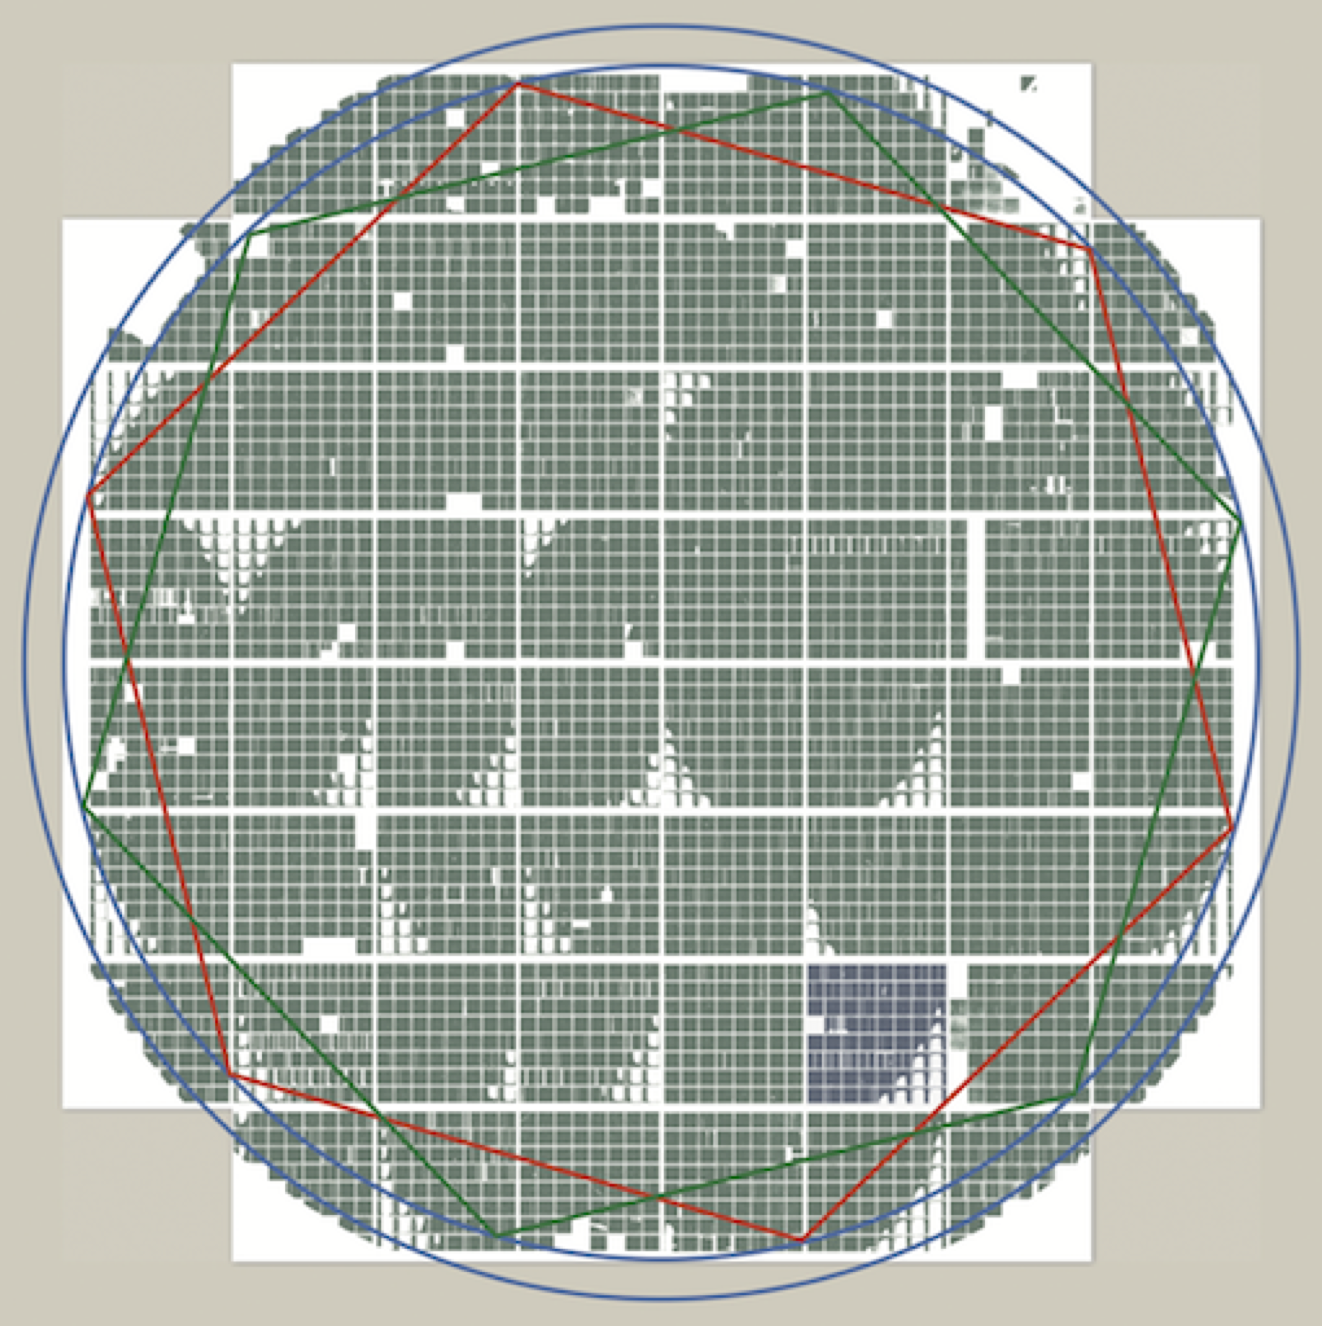
\includegraphics[width=\textwidth]{../figures/05_sedfit/GPC1focalplan.png}
  \end{minipage}\hfill
  \begin{minipage}[c]{0.5\textwidth}
    \caption[Plan focal de la Gigapixel Camera (PS1)]{Plan focal de la
    Gigapixel Camera (PS1) (figure de \citet{ChambersPS1survey}). Les cellules non fonctionnelles sont
    masquées et représentées en blanc dans la figure ci-dessus.}\label{fig:gpc1focalplan}
  \end{minipage}
\end{figure}


Une des missions de PS1 (à plus de $56\%$ du temps alloué) est l'observation de tout le ciel Nord à une déclinaison $\delta>30\degree$ :
c'est le
relevé $3\pi$ Stéradian. Les observations sont effectuées avec 5 filtres
$g_{P1}$, $r_{P1}$, $i_{P1}$, $z_{P1}$ et $y_{P1}$. On notera
l'existence d'un  sixième
filtre ($w_{P1}$) qui
englobe les filtres $g,r,i$ mais qui est utilisé pour l'étude du système
solaire et non le relevé $3\pi$ Stéradian. Les informations
de transmission de ces $6$ filtres sont présentées dans la Figure~\ref{fig:ps1filters}.

\begin{figure}
  \centering
  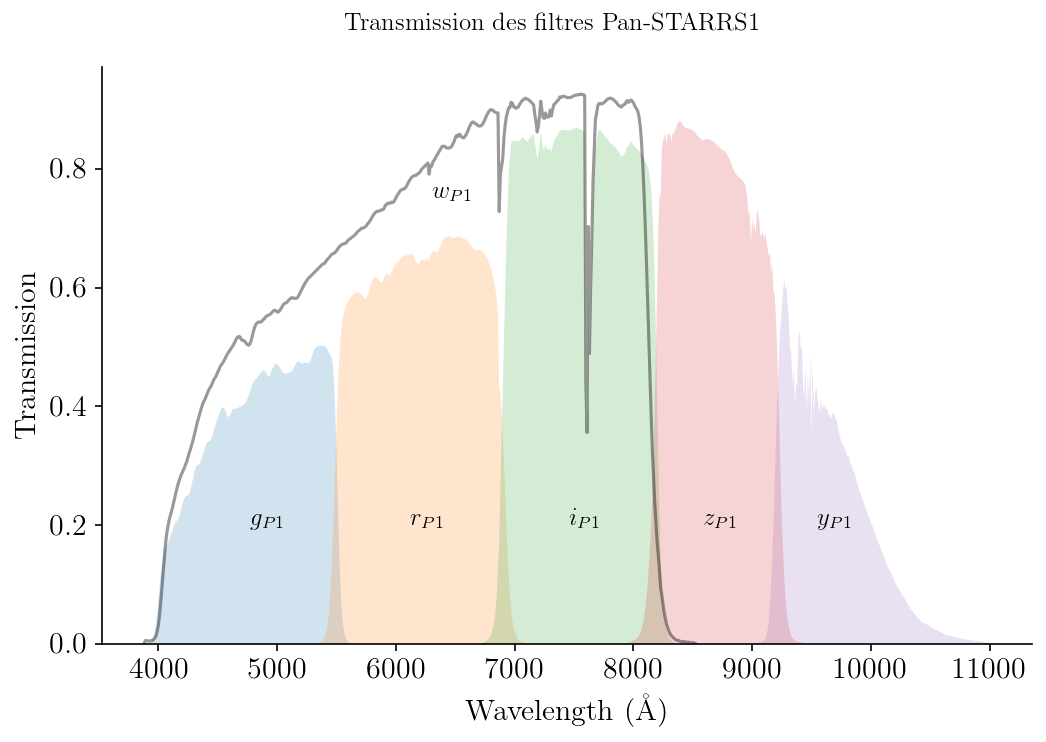
\includegraphics[width=0.8\textwidth]{../figures/05_sedfit/ps1filters.png}
  \caption[Transmission des filtres Pan-STARRS1]{Transmission des
    filtres $grizy$ de Pan-STARRS1.}
  \label{fig:ps1filters}
\end{figure}


Pan-STARRS1 utilise le système de magnitude ``AB'' \citep{Oke1983}
décrit en détail pour le relevé SDSS \citep{YorkSDSS2000} par
\citet{Fukugita1996}.

Dans ce système, une magnitude monochromatique AB est défini comme le
logarithme de la densité spectrale de flux, tel que:

\begin{align}
  \label{eq:abmag}
  m_{AB}(\nu)&= -2.5\log_{10}(f_{\nu}[\erg\ \text{s}^{-1}\cm^{-2}\Hz^{-1}]) -
  48.60\\
  m_{AB}(\nu)&\approx -2.5\log_{10}(\frac{f_{\nu}[\jy]}{3631\jy})
\end{align}

Avec $1\text{Jy} = 10^{-23}\erg.\sec^{-1}\cm^{-2}\Hz^{-1}$.

La magnitude AB d'une bande passante est alors définie telle que:
\begin{equation}
  \label{eq:abmagbp}
  m_{AB}\approx-2.5\log_{10}\left(\frac{\int
      f_{\nu}(h\nu)^{-1}A(\nu)\d\nu}{\int 3631\jy(h\nu)^{-1}A(\nu)\d\nu}   \right)
\end{equation}

Où $A(\nu)$ est la fonction de réponse du filtre considéré. Le système
photométrique de PS1 est détaillé dans \citet{Tonry2012}.

\begin{table}[h]
    \centerfloat
    \begin{threeparttable}
        \caption{Caractéristiques des filtres $grizy$ de PAN-STARRS1 et
          du relevé $3\pi$ Stéradian.}
        \label{tab:3pisteradian}
        \begin{tabular}{lccccccc}
            \toprule
             \multirow{2}[3]{*}{Filtres} & \multirow{2}[3]{*}{$\lambda_{pivot}$(\AA)} &                                                                    \multirow{2}[3]{*}{\# Expositions}  & \multirow{2}[3]{*}{\shortstack{mag
                                                  à $5\sigma$ \\(exposition unique)}} &
                                                                 \multirow{2}[3]{*}{\shortstack{mag
                                  à $5\sigma$ \\
          (expositions empilées)}} & \multirow{2}[3]{*}{\shortstack{Median
                                  \\seeing ('') }} &  \multirow{2}[3]{*}{\shortstack{Mode
                                  \\seeing ('')}} \\
          \\
            & & & & & & \\
          \midrule
          $g_{P1}$ & $4849.11$ &60528 & $22.0$ & $23.3$ & $1.47$ & $1.31$\\
          $r_{P1}$ & $6201.20$ &70918 & $21.8$ & $23.2$ & $1.31$ & $1.15$\\
          $i_{P1}$ & $7534.96$ &104414& $21.5$ & $23.1$ & $1.19$ & $1.05$\\
          $z_{P1}$ & $8674.20$ &67604 & $20.9$ & $22.3$ & $1.14$ & $1.00$\\
          $y_{P1}$ & $9627.79$ &70982 & $19.7$ & $21.4$ & $1.09$ & $0.95$\\
                     
            \bottomrule
        \end{tabular}
        \begin{tablenotes}[flushleft]
        \item \textbf{Notes.} La longueur d'onde pivot $\lambda_{pivot}$
          est déterminée avec la transmission $T(\lambda)$ tel que
          $\lambda_{pivot}=\sqrt{\frac{\int T(\lambda)\d\lambda}{\int T(\lambda)\d\lambda/\lambda^{2}}}$
        \end{tablenotes}
    \end{threeparttable}
\end{table}


Nous présentons dans la Table\ref{tab:3pisteradian} quelques
caractéristiques des filtres $grizy$ de PS1, ainsi que du relevé $3\pi$
Stéradian.

\subsection{Utilisation des images PS1}
\label{ssec:preprocessps1}

Bien entendu nous n'utilisons pas les images brutes acquisent par PS1,
mais celles ayant été traitées avec différentes étapes de corrections,
qui constituera in fine la $1\iere$ Data Release de PS1.

Ces étapes de traitement d'image sont détaillées dans
\citet{Waters2020}.

La section 3 de \citet{Waters2020} décrit la partie corrective des
images:

\begin{itemize}[label=$\diamondsuit$]
  \itemsep0em 
   \item \textbf{Soustraction du bias et du dark} pour prendre en compte le bruit
     de lecture et le bruit thermique en fonction du temps d'exposition.
   \item \textbf{Cartographie du bruit} (qui n'est pas forcément uniforme, mais peut
     présenter un gradient).
   \item \textbf{Division du flat} pour corriger les effets de vignettage. Les
     flats sont pris avec une exposition du ciel à l'aube ou au
     crépuscule.
   \item  \textbf{Correction d'effets de franges} dans les images. Ces structures
     d'interférences sont notamment visibles vers l'infrarouge, où les
     longueurs d'ondes sont du même ordre de grandeur que l'épaisseur du
     détecteur.
   \item \textbf{Application d'un masque statique} pour les pixels du détecteur
     défectueux ou ayant une réponse très faible dans toutes les expositions, et un \textbf{masque dynamique}
     qui va varier pour chaque observation.
   \item \textbf{Correction d'effet de persistence}, dû à la saturation d'un
     pixel. Ce phénomène créé une trainée verticale partant du centre de
     la source de forte luminosité.
   \item \textbf{Correction des non-linéarités}, les pixels de la GPC1
     n'ayant pas une réponse uniformément linéaire en fonction du niveau
     de flux. Ce phénomène est d'autant plus prononcé aux bords du
     détecteur et à bas flux.
   \item \textbf{Correction de motifs} notamment horizontaux dus à des
     effets de 
     diaphonies entre deux lignes de pixels adjacentes.
   \item \textbf{Modélisation et soustraction du fond du ciel}, une fois
     que toutes les corrections précédentes ont été appliquées.
\end{itemize}

L'étape suivante de traitement des images, décrite dans la section 5 de
\citet{Waters2020}, est une transformation géométrique, passant de l'espace du
plan focal en un système de pixels cohérent vis à vis d'une localisation donnée
du ciel. Cette transformation permet alors d'effectuer des opérations de
combinaisons d'images superposants une partie commune du ciel. Dans ce
nouveau système d'agencement, les pixels ont alors une taille de
$0\farcs25$ de côté.


La section 6 de \citet{Waters2020} traite justement de la procédure
d'empilement d'images, permettant ainsi un meilleur ratio signal sur
bruit (SNR) dans les zones du ciel communes à plusieurs expositions. Cet
empilement est effectué de sorte que toutes les images aient un point
zero de $ZP=\SI{25.0}{mag}$, et un airmass de $\chi=1$. Ce
sont ces images traitées et empilées que nous utiliserons pour la
modélisation hyperspectrale des galaxies hôtes.


Nous utilisons pour cela le serveur libre d'accès aux images
PS1\footnote{\url{https://ps1images.stsci.edu/cgi-bin/ps1cutouts}},
permettant d'effectuer une requête d'images centrées sur une position du
ciel arbitraire (RA, DEC), et de côté arbitraire X pixels, sachant que chaque pixel
est de forme carré de $0\farcs25$ de côté. Les images peuvent être
récupérées dans chacun des 5 filtres $g_{P1}$, $r_{P1}$, $i_{P1}$,
$z_{P1}$ et/ou $y_{P1}$, avec un flux par pixel exprimé en unité de coups. Nous montrons dans la
Figure~\ref{fig:pscutoutsZTF18accrorf} une image de $140\times140$
pixels ($=35"\times35"$) centrée sur la position de détection par ZTF de
ZTF18accrorf. 

\begin{figure}[ht]
  \begin{minipage}[c]{0.45\textwidth}
    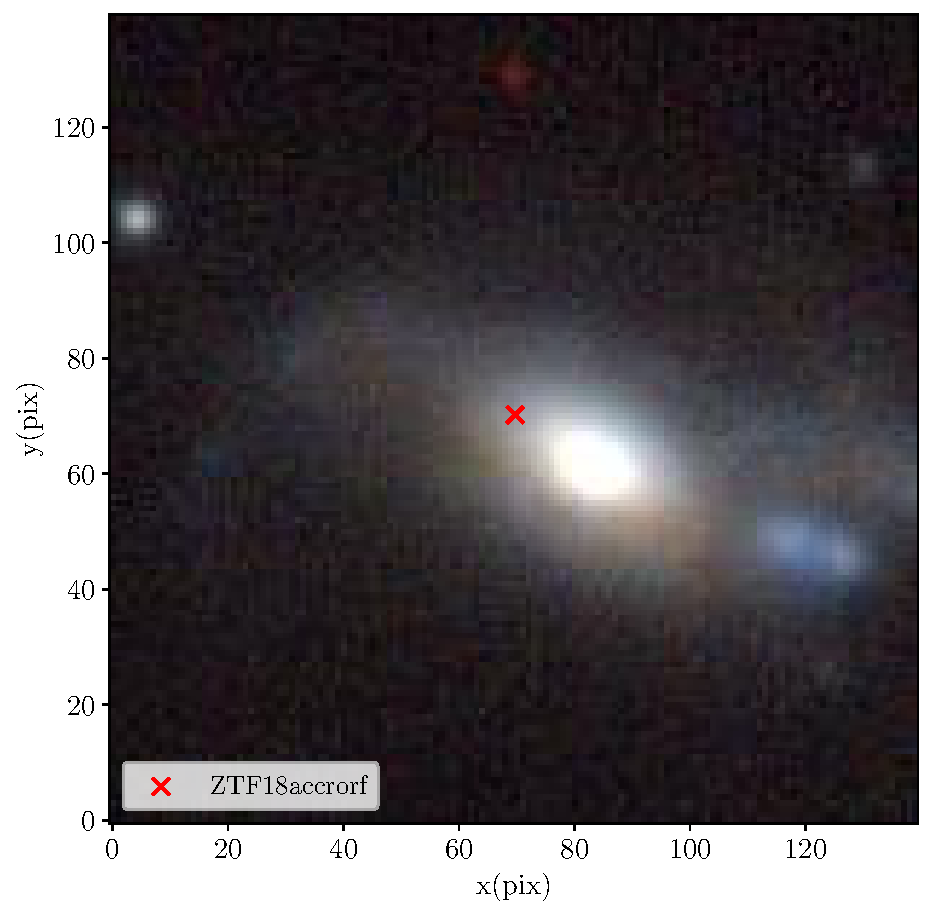
\includegraphics[width=\textwidth]{../figures/05_sedfit/ps_cutouts_ZTF18accrorf.pdf}
  \end{minipage}\hfill
  \begin{minipage}[c]{0.52\textwidth}
    \caption[Image RGB de PS1 centrée sur ZTF18accrorf.]{Image RGB
      construite à partir des bandes $g_{P1}$, $r_{P1}$ et
      $z_{P1}$ des images PS1. L'image fait $35"$ de côté et est centrée sur la position de
      détection de ZTF18accrorf par ZTF, à $(\text{RA}, \text{DEC})=(17.1692\degree,20.0799\degree)$}\label{fig:pscutoutsZTF18accrorf}
  \end{minipage}
\end{figure}


\section{\pkg{Cigale} et SEDFitting}
\label{sec:cigale}

Ayant à présent accès aux images photométriques contenant le champ
de vue de l'IFU de la SEDm, nous pouvons passer à l'étape suivante de
notre raisonnement, à savoir la modélisation hyperspectrale. Pour cela,
nous avons vu dans le chapitre précédent qu'il nous faut un outil
permettant d'interpoler une SED à partir des données
photométriques: un SED Fitter. 

\subsection{Présentation de \pkg{Cigale}}
\label{ssec:cigale}

\pkg{Cigale}, pour Code Investigating GALaxy Emission, est un modéliseur
de SED basé sur une approche Bayesienne et écrit initialement en \pkg{FORTRAN} par \citet{Noll2009,Burgarella2005}. 
Le code a ensuite été étendu avec de nombreux modules
supplémentaires et
entièrement réadapté en \pkg{PYTHON} par \citet{Boquien2019}. 

L'idée générale est la construction dans un premier temps du modèle de
population stellaire, puis d'ajouter les effets d'absorption par la
poussière et les émissions nébulaires. Enfin, par conservation
d'énergie, l'énergie absorbée par la poussière dans à basses longueurs
d'onde est réémise dans l'infrarouge.

La méthode de modélisation est basée sur un calcul progressif via
l'utilisation d'une succession de modules,
chacun correspondant à une unique composante ou processus physique. Pour
chaque module, un set de paramètres est fixé par l'utilisateur. Le code
va ainsi explorer la totalité des combinaisons possibles entres
tous les modules et leur liberté via ces paramètres, où chaque
combinaison résultera en un modèle différent de SED.

La séquence de détermination d'un modèle se fait par les calculs suivants
(section 3 de \citet{Boquien2019}) :

\begin{enumerate}
\item Histoire de la formation stellaire (SFH) de la galaxie.
\item Spectre stellaire à partir de la SFH et du modèle de
  population stellaire choisi par l'utilisateur.
\item Emission nébulaire (continuum et raies d'émission).
\item Atténuation des émissions stellaires et nébulaires suivant la
    loi d'atténuation utilisée (également fixée par l'utilisateur), puis
    calcul de la luminosité absorbée par la pousière.
\item En se basant sur le principe d'équilibre énergétique, calcul de
    l'émission par la poussière dans l'infrarouge  moyen et lointain
    (énergie réémise à partir de celle absorbée aux courtes
    longueurs d'onde - étape précédente).
\item Emission d'un noyau actif.
\item Décalage vers le rouge des modèles suivant le redshfit
      d'entrée renseigné au préalable, et calcul de l'absorption du
      milieu inter-galactique.
  
\end{enumerate}

Nous ne détaillerons pas ici la technicité de la méthode Bayesienne ni
la description de chacun des modules que propose \pkg{CIGALE} tant ils
sont nombreux. Nous nous focaliserons donc sur l'utilisation que nous faisons
de ce modéliseur de SED et son application sur les images photométriques
de PS1.

\subsection{Préparation des images photométriques}
\label{ssec:preprocessimages}


\begin{figure}
  \centering
  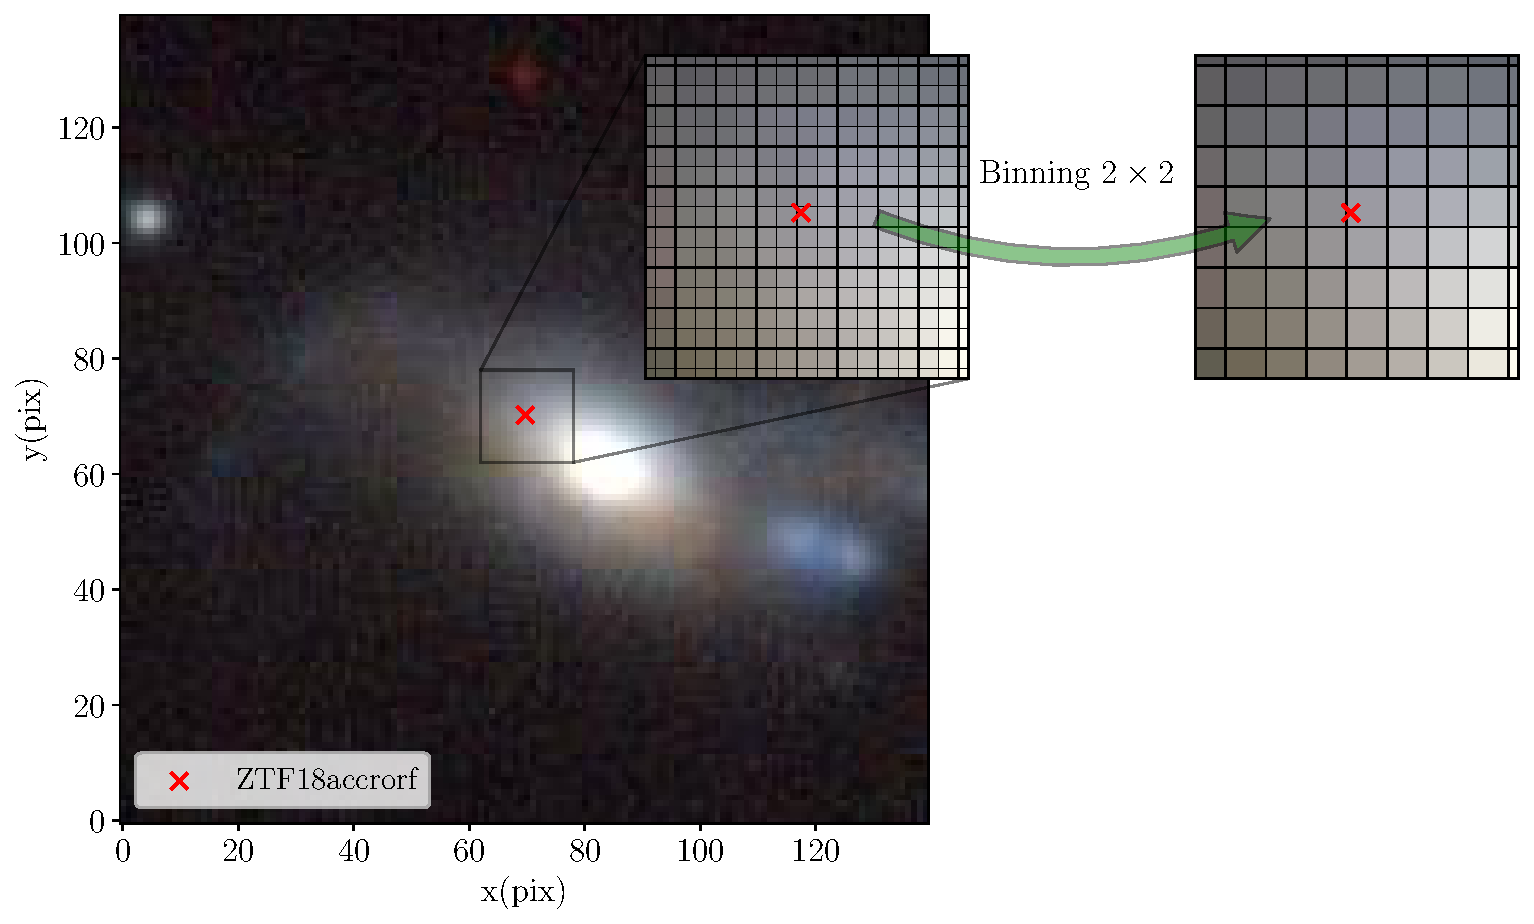
\includegraphics[width=0.99\textwidth]{../figures/05_sedfit/ps_cutouts_ZTF18accrorf_binned.pdf}
  \caption[Illustration binning $2\times2$ sur les images PS1.]{Image RGB
      construite à partir des bandes $g_{P1}$, $r_{P1}$ et
      $z_{P1}$ des images PS1. L'image fait $35"$ de côté et est centrée sur la position de
      détection de ZTF18accrorf par ZTF, à $(\text{RA}, \text{DEC})=(17.1692\degree,20.0799\degree)$}
  \label{fig:pscutoutsZTF18accrorf_binned}
\end{figure}

\subsection{Configuration et utilisation de \pkg{CIGALE}}
\label{ssec:cigaleconfig}


\section{Construction du cube intrinsèque}

\subsection{Sampling des spectres dans l'espace SEDm}
%\label{ssec:xxx}

\subsection{Construction du cube}
% \label{ssec:xxx}

\bibliographystyle{../main/aa_url2}
\bibliography{99_references}

\end{document}

%%% Local Variables:
%%% mode: latex
%%% TeX-master: t
%%% End:
